\documentclass[11pt]{article}
\usepackage{amsmath, amssymb, amsthm}
\usepackage{booktabs}
\usepackage{geometry}
\usepackage{enumitem}
\usepackage{caption}
\usepackage{mathtools}
\usepackage{fontawesome5}
\usepackage{hyperref}  % MUST be loaded for \texorpdfstring
\geometry{margin=1in}



\usepackage{tikz}
\usetikzlibrary{positioning}


\title{Mutual Information of Dependent Random Variables}
\author{}
\date{}

\begin{document}

\maketitle

\Large

\section{Probability Theory}

In this section we give a quick recap of some important ideas from probability theory. We will be focusing on the discrete case.

\subsection{Events and Random Variables}


The first important point is to distinguish between an \emph{event} in some sample space $\Omega$ and a \emph{random variable} $X: \Omega \to \mathbb{R}$ which assigns real values to outcomes.


Let $\Omega$ denote the sample space of all possible outcomes of an experiment. An \textbf{event} is any subset of $\Omega$ . It represents a collection of outcomes about which we are interested. 

For example, consider tossing a fair coin twice. The sample space is
\[
\Omega = \{ HH, HT, TH, TT \}.
\]
The event
$
A = \{\text{exactly one head}\} = \{ HT, TH \}
$
is a subset of $\Omega$. Since the coins are both fair, the probability of this event is:
\[
P(A) = P(\{HT, TH\}) = \frac{1}{4} + \frac{1}{4} = \frac{1}{2}.
\]

A \textbf{random variable} $X$ is a function
\[
X : \Omega \to \mathbb{R}
\]
that assigns a numerical value to each outcome in the sample space. When we write $X = x$, we are referring to the \emph{event} consisting of all outcomes $\omega \in \Omega$ for which $X(\omega) = x$:
\[
\{ \omega \in \Omega : X(\omega) = x \}.
\]
For example, let $X = \#\text{heads in two tosses}$. Then
\[
X(HH) = 2, \quad X(HT) = 1, \quad X(TH) = 1, \quad X(TT) = 0.
\]
The statement $X = 1$ corresponds to the event
\[
\{\omega \in \Omega : X(\omega) = 1\} = \{ HT, TH \},
\]
which is exactly the same event as $A$ in the previous example. Thus, a random variable taking on a particular value is just a special kind of event.

We may use the notation: \[P_X(1) = \frac{1}{2}\]

To summarize: An \textbf{event} is a subset of the sample space, representing outcomes of interest. A \textbf{random variable taking a value} defines an event consisting of all outcomes that map to that value. 


\subsection{Conditional Probability, Independence and Bayes Theorem}


The \textbf{conditional probability} of $A$ given $B$ is defined as:
\[
P(A \mid B) = \frac{P(A \cap B)}{P(B)}, \quad \text{for } P(B) > 0.
\]
Equivalently,
\[
P(B \mid A) = \frac{P(A \cap B)}{P(A)}, \quad \text{for } P(A) > 0.
\]


Setting the two different expressions for $P(A \cap B)$ equal to each other in the above equations gives us \textbf{Bayes' theorem}:
\[
\boxed{
P(A \mid B) = \frac{P(B \mid A) \, P(A)}{P(B)}, \quad \text{for } P(B) > 0
}
\]


For random variables $X$ and $Y$ the notation for conditional probability looks like:
    \[
    P_{X \mid Y}(x \mid y) = \frac{P_{X,Y}(x,y)}{P_Y(y)}, \quad P_Y(y) > 0.
    \]
    In this case, $X=x$ and $Y=y$ are themselves events in $\Omega$, and $P_{X \mid Y}(x \mid y)$ measures the probability that $X$ takes value $x$ given that $Y$ takes value $y$.
    
    In this notation Bayes' theorem looks like:
    \begin{equation*} \boxed{
P_{X \mid Y}(x \mid y) = \frac{P_{Y \mid X}(y \mid x) \, P_X(x)}{P_Y(y)} }
\end{equation*}


Two \textbf{events} $A$ and $B$ are \emph{independent} if:
\[
P(A \cap B) = P(A) \, P(B)
\]
Otherwise, for dependent events, we have:
\[
P(A \cap B) = P(A) \, P(B \mid A) = P(B) \, P(A \mid B)
\]
Equivalently, $A$ and $B$ are independent if knowing one tells you nothing about the other:
\[
P(B) = P(B \mid A) \quad \text{or equivalently} \quad P(A) = P(A \mid B)
\]






\subsection{Example of Dependent Events}

Consider rolling two fair six-sided dice.

Define the events:
\[
A = \{\text{sum of the dice is even}\}, \quad
B = \{\text{sum of the dice is greater than 7}\}
\]
There are 36 equally likely outcomes.
The probabilities are calculated as follows:
\begin{itemize}
    \item $P(A) = \frac{18}{36} = 0.5$
    \item $P(B) = \frac{15}{36} \approx 0.4167$
    \item $P(A \cap B) = \frac{9}{36} = 0.25$.
\end{itemize}
To check for independence, we compute the product:
\[
P(A)P(B) = 0.5 \cdot \frac{15}{36} \approx 0.2083
\]
Since $0.25 \neq 0.2083$, $P(A \cap B) \neq P(A)P(B)$, and the events $A$ and $B$ are \textbf{dependent}.

The conditional probability $P(A \mid B) = \frac{P(A \cap B)}{P(B)} = \frac{0.25}{0.4167} \approx 0.6$. 

Since $P(A \mid B) > P(A)$, knowing that the sum is greater than 7 increases the probability that the sum is even, confirming dependence.



\subsection{Another Example of Dependent Events}
Define the events:
\[
C = \{\text{at least one die shows 6}\}, \quad
D = \{\text{sum of the dice is greater than 10}\}
\]
The probabilities are:
\begin{itemize}
    \item $P(C) = \frac{11}{36} \approx 0.3056$
    \item $P(D) = \frac{3}{36} \approx 0.0833$
    \item $P(C \cap D) = \frac{3}{36} \approx 0.0833$.
\end{itemize}
To check for independence, we compare $P(C \cap D)$ with $P(C)P(D)$:
\[
P(C)P(D) = \frac{11}{36} \cdot \frac{3}{36} = \frac{33}{1296} \approx 0.0254
\]
Since $0.0833 \neq 0.0254$, $P(C \cap D) \neq P(C)P(D)$, and the events $C$ and $D$ are \textbf{dependent}.

The conditional probability $P(D \mid C) = \frac{P(C \cap D)}{P(C)} = \frac{0.0833}{0.3056} \approx 0.2727$. 

Since $P(D \mid C) > P(D)$, knowing that one die is a 6 significantly increases the probability of a sum greater than 10, demonstrating dependence.













\section{Coin Tossing Experiment}

We toss a fair coin \textbf{twice}. The four possible \textbf{elementary outcomes} (or \emph{events}) are:
\begin{itemize}
    \item \textbf{HH}: heads then heads  
    \item \textbf{HT}: heads then tails  
    \item \textbf{TH}: tails then heads  
    \item \textbf{TT}: tails then tails
    \end{itemize}
Each occurs with probability $ \frac{1}{4} $, since the coin is fair and tosses are independent.
From these raw outcomes, we define two \textbf{random variables}—that is, numerical summaries:

\begin{itemize}
    \item Let \textbf{$X$} be the difference between the number of heads and tails:
    \[
    X = (\#\text{heads}) - (\#\text{tails})
    \]
    So:
        \item HH $\to X = 2 - 0 = +2$
        \item HT or TH $\to X = 1 - 1 = 0$
        \item TT $\to X = 0 - 2 = -2$

    \item Let \textbf{$Y$} indicate whether the two tosses \textbf{match}:
    \[
    Y = 
    \begin{cases}
    +1 & \text{if both tosses are the same (HH or TT)} \\
    -1 & \text{if they differ (HT or TH)}
    \end{cases}
    \]
\end{itemize}

It is important not to confuse the \emph{outcomes} and the \emph{random variables}. The \textbf{underlying events} are HH, HT, TH, TT, the \textbf{random variables} $X$ and $Y$ assign numbers to the underlying events in such a way that multiple events can lead to the same $(X,Y)$ pair.

\begin{center}
\begin{tabular}{lccc}
\toprule
Event & $X$ & $Y$ & Probability \\
\midrule
HH    & $+2$   & $+1$   & $1/4$     \\
HT    & $0$    & $-1$   & $1/4$     \\
TH    & $0$    & $-1$   & $1/4$     \\
TT    & $-2$   & $+1$   & $1/4$     \\
\bottomrule
\end{tabular}
\end{center}

Notice that \textbf{HT and TH both give $(X=0, Y=-1)$}, so their probabilities add:
 \begin{itemize}
    \item $P(X = 0, Y = -1) = \frac{1}{4} + \frac{1}{4} = \frac{1}{2}$
    \item $P(X = +2, Y = +1) = \frac{1}{4}$
    \item $P(X = -2, Y = +1) = \frac{1}{4}$
\end{itemize}
All other $(x,y)$ pairs have probability 0.


We can now build the \textbf{joint probability distribution} $P_{X,Y}(x, y) = \mathbb{P}(X = x \text{ and } Y = y)$. After grouping outcomes that lead to the same 
$(X,Y)$ pair, the joint probability distribution of the random variables is:

\begin{center}
\begin{tabular}{ccc}
\toprule
X & Y & $P(X,Y)$ \\
\midrule
+2 & +1 & 1/4 \\
0  & -1 & 1/2 \\
-2 & +1 & 1/4 \\
\bottomrule
\end{tabular}
\end{center}
This will be useful later for calculating the conditional entropy later on.

\newpage

\section*{Entropy}

\subsection*{Information Content of a Single Outcome}

For a random variable $X$ with possible outcome $x$ and probability $P_X(x)$, the \textbf{information content} (or \emph{self-information}) of observing $x$ is defined as:
\[
I(x) = - \log_2 P_X(x)
\]

Intuitively:
\begin{itemize}
    \item Rare events (small $P_X(x)$) are more \textbf{surprising} and carry more information.  
    \item Common events (large $P_X(x)$) are less surprising and carry less information.  
\end{itemize}

\subsection*{Example 1: Fair Coin}

A fair coin has:
\[
P(\text{Heads}) = P(\text{Tails}) = 1/2
\]

\[
I(\text{Heads}) = I(\text{Tails}) = - \log_2(1/2) = 1 \text{ bit}
\]

Each flip of a fair coin provides 1 bit of information on average.

\subsection*{Example 2: Biased Coin}

Consider a biased coin with:
\[
P(\text{Heads}) = 0.9, \quad P(\text{Tails}) = 0.1
\]

Information content of each outcome:
\[
I(\text{Heads}) = - \log_2 0.9 \approx 0.152 \text{ bits}, \quad
I(\text{Tails}) = - \log_2 0.1 \approx 3.32 \text{ bits}
\]

Observing \textbf{Heads} is unsurprising and carries very little information, while observing \textbf{Tails} is rare and highly informative.

\subsection*{Entropy: Average Information}

The \textbf{entropy} of a random variable $X$ measures the \textbf{average information content} over all outcomes:
\[
H(X) = \mathbb{E}[I(X)] = - \sum_x P_X(x) \log_2 P_X(x)
\]

Entropy quantifies the \emph{expected surprise} or \emph{uncertainty} before observing the outcome.

\subsubsection*{Fair Coin}

\[
H(X) = - \left( \frac{1}{2} \log_2 \frac{1}{2} + \frac{1}{2} \log_2 \frac{1}{2} \right) = 1 \text{ bit}
\]

\subsubsection*{Biased Coin}

\[
H(X) = - \left(0.9 \log_2 0.9 + 0.1 \log_2 0.1 \right) \approx 0.61 \text{ bits}
\]

Because the biased coin outcome is more predictable, each flip provides less information on average than a fair coin.

\subsection*{Summary}

\begin{itemize}
    \item \textbf{Information} measures the surprise of a single outcome.  
    \item \textbf{Entropy} measures the \textbf{average information} across all outcomes.  
    \item High entropy = outcomes are uncertain (fair coin).  
    \item Low entropy = outcomes are predictable (biased coin).  
\end{itemize}








\section*{Additivity}

Because of the logarithm, entropy is additive. If $X$ and $Y$ are independent then:
\[
H(X, Y) = H(X) + H(Y)
\]
The unit of entropy is the \textbf{bit}.

If we flip $n$ independent fair coins $X_1, X_2, \dots, X_n$, the total entropy is additive:
\[
H(X_1, X_2, \dots, X_n) = H(X_1) + H(X_2) + \dots + H(X_n) = n \text{ bits}.
\]

Intuitively, additivity works because independent variables carry \emph{separate, non-overlapping information}. 
If the variables are \textbf{not independent}, knowing one gives partial information about the other, so the joint entropy is less than the sum:
\[
H(X, Y) < H(X) + H(Y) \quad \text{if $X$ and $Y$ are dependent.}
\]
We will see concrete examples of this later.


Back to our example, for $X$, which takes values $-2, 0, +2$ with probabilities $\frac{1}{4}, \frac{1}{2}, \frac{1}{4}$, we compute:
\[
\begin{aligned}
H(X) &= -\sum_x P_X(x) \log_2 P_X(x) \\
&= -\left[ \frac{1}{4} \log_2 \frac{1}{4} + \frac{1}{2} \log_2 \frac{1}{2} + \frac{1}{4} \log_2 \frac{1}{4} \right] \\
&= -\left[ \frac{1}{4}(-2) + \frac{1}{2}(-1) + \frac{1}{4}(-2) \right] = -[-1.5] = 1.5
\end{aligned}
\]
So \textbf{$H(X) = \frac{3}{2}$ bits}. 

Now let's calculate the entropy of $Y$

$Y$ can take either of the values $+1$ or $-1$, each with probability $\frac{1}{2}$, so:
\[
H(Y) = -\left[ \frac{1}{2} \log_2 \frac{1}{2} + \frac{1}{2} \log_2 \frac{1}{2} \right] = 1 \text{ bit}
\]
Knowing nothing, it takes 1 bit to describe whether the tosses matched.

\section*{Conditional Entropy $H(X \mid Y)$}

We are now working with \textbf{non-independent} random variables. Suppose we \textbf{first learn the value of $Y$}. How much uncertainty about $X$ remains?

First, we define the \textbf{conditional entropy for a specific value of $Y$}:

\[
H(X \mid Y = y) = - \sum_x P_{X \mid Y}(x \mid y) \, \log_2 P_{X \mid Y}(x \mid y),
\]

where the \textbf{conditional probability} is
\[
P_{X \mid Y}(x \mid y) = \frac{P_{X,Y}(x, y)}{P_Y(y)}, \quad \text{for } P_Y(y) > 0.
\]

\noindent In words: 

The conditional probability $P_{X \mid Y}(x \mid y)$ gives the probability that $X = x$ 
 given that $Y = y$. It is computed by dividing the joint probability $P_{X,Y}(x,y)$ 
by the marginal probability $P_Y(y)$.


The \textbf{conditional entropy of $X$ given $Y$} is then the \emph{average} of $H(X \mid Y = y)$ over all possible values of $Y$, weighted by their probabilities:

\[
H(X \mid Y) = \sum_y P_Y(y) \, H(X \mid Y = y).
\]

This expresses that the conditional entropy is the \textbf{average remaining uncertainty about $X$} once we know $Y$.







We are working now with non-independent random variables. Suppose we \textbf{first learn the value of $Y$}. How much uncertainty about $X$ remains?

Let us first define:
\[
H(X \mid Y = y) = - \sum_x P_{X \mid Y}(x \mid y) \, \log_2 P_{X \mid Y}(x \mid y)
\]
where:
\[
P_{X \mid Y}(x \mid y) = \frac{P_{X,Y}(x, y)}{P_Y(y)}, \quad \text{for } P_Y(y) > 0
\]

\[\text{The conditional probability } P_{X \mid Y}(x \mid y) \text{ is the probability that } X = x 
\text{ given that } Y = y. \text{ It is calculated by dividing the joint probability } 
P_{X,Y}(x,y) \text{ by the marginal probability } P_Y(y).\]


We now have the definition:
\[
H(X \mid Y) = \sum_y P_Y(y) \cdot H(X \mid Y = y)
\]
This says that the conditional entropy 
is the average uncertainty remaining about 
$X$
once we know 
$Y$
averaged over all possible values that 
$Y$
can take, weighted by their probabilities."

\subsection*{When $Y = +1$ (tosses match $\to$ HH or TT):}
\begin{itemize}
    \item This happens with probability $P_Y(+1) = \frac{1}{2}$
    \item Given this, $X = +2$ (HH) or $X = -2$ (TT), each with conditional probability:
    \[
    P(X = +2 \mid Y = +1) = \frac{P(X=+2, Y=+1)}{P_Y(+1)} = \frac{1/4}{1/2} = \frac{1}{2}
    \]
    (same for $X = -2$)
    \item So the conditional entropy is:
    \[
    H(X \mid Y = +1) = -\left[ \frac{1}{2} \log_2 \frac{1}{2} + \frac{1}{2} \log_2 \frac{1}{2} \right] = 1 \text{ bit}
    \]
\end{itemize}
\subsection*{When $Y = -1$ (tosses differ $\to$ HT or TH):}
\begin{itemize}
    \item Probability $P_Y(-1) = \frac{1}{2}$
    \item Both HT and TH give $X = 0$, so:
    \[
    P(X = 0 \mid Y = -1) = 1
    \]
    \item Thus:
    \[
    H(X \mid Y = -1) = -[1 \cdot \log_2 1] = 0 \text{ bits}
    \]
\end{itemize}

\subsection*{Average over $Y$:}
\[
H(X \mid Y) = \frac{1}{2} \cdot 1 + \frac{1}{2} \cdot 0 = \frac{1}{2} \text{ bit}
\]
On average, once we know whether the tosses matched, we only need \textbf{half a bit more} to pin down $X$.

\section*{{Step 4} Mutual Information $I(X; Y)$}

\textbf{Mutual information} answers:  
``How many bits of uncertainty about $X$ are \textbf{removed} by knowing $Y$?''  
Or equivalently: ``How much do $X$ and $Y$ tell us about each other?''

Mathematically:
\[
I(X; Y) = H(X) - H(X \mid Y)
\]

Plugging in:
\[
I(X; Y) = \frac{3}{2} - \frac{1}{2} = 1 \text{ bit}
\]

We can \textbf{verify this another way}: check $H(Y \mid X)$.

\begin{itemize}
    \item If $X = 0$ $\to$ must be HT or TH $\to$ $Y = -1$ for sure
    \item If $X = +2$ $\to$ must be HH $\to$ $Y = +1$
    \item If $X = -2$ $\to$ must be TT $\to$ $Y = +1$
\end{itemize}
So \textbf{knowing $X$ tells us $Y$ exactly} $\to$ $H(Y \mid X) = 0$

Thus:
\[
I(X; Y) = H(Y) - H(Y \mid X) = 1 - 0 = 1 \text{ bit}
\]

Both ways agree.

\textbf{Interpretation}: $X$ and $Y$ share \textbf{1 bit of information}.  
In fact, $Y$ is a \textbf{function of $X$} (you can compute matching status from the head--tail difference), so all of $Y$'s information is contained in $X$. But $X$ has extra detail (sign of the difference) that $Y$ doesn't capture—which is why $H(X) > H(Y)$.

\section*{{Final Results}}

\begin{center}
\begin{tabular}{lc}
\toprule
Quantity & Value \\
\midrule
$H(X)$ & $1.5$ bits \\
$H(Y)$ & $1$ bit \\
$H(X \mid Y)$ & $0.5$ bits \\
$H(Y \mid X)$ & $0$ bits \\
$I(X; Y)$ & $1$ bit \\
\bottomrule
\end{tabular}
\end{center}

\section*{{Key Takeaway}}

Even though we started with \textbf{four equally likely physical outcomes} (HH, HT, TH, TT), the random variables $X$ and $Y$ \textbf{compress} this information in different ways.
 \begin{itemize}
    \item $X$ distinguishes \textbf{three cases} (++ , +--/--+ , --)
    \item $Y$ distinguishes \textbf{two cases} (same vs. different)
Their \textbf{mutual information} quantifies exactly how much these summaries overlap—and in this case, \textbf{all of $Y$'s content is inside $X$}, but not vice versa.
\end{itemize}

This is the power of information theory: it lets us \textbf{measure shared knowledge} between any two descriptions of the same experiment—whether they’re numbers, categories, or even words.

\newpage








\newpage







\section*{\texorpdfstring{\faLightbulb}{Intuition} What Is Conditional Entropy?}

\textbf{Conditional entropy} \(H(X \mid Y)\) quantifies the \textbf{average remaining uncertainty} in a random variable \(X\) after the value of another random variable \(Y\) has been observed. In other words, it answers:

\begin{quote}
``If I know \(Y\), how much don’t I still know about \(X\)—on average?''
\end{quote}

It is always true that \(H(X \mid Y) \leq H(X)\), with equality if and only if \(X\) and \(Y\) are statistically independent.

\section*{\texorpdfstring{\faKey}{Key Building Block} Joint Probability}

Before defining conditional entropy, we need the \textbf{joint probability distribution} of \(X\) and \(Y\):

\[
\boxed{P_{X,Y}(x, y) = \mathbb{P}(X = x \text{ and } Y = y)}
\]

This is the probability that \textbf{both} \(X\) takes the value \(x\) \textbf{and} \(Y\) takes the value \(y\) in the same trial of the experiment. The joint distribution fully describes how \(X\) and \(Y\) behave together.

From it, we obtain the \textbf{marginal distributions} by summing out the other variable:
\[
P_X(x) = \sum_{y} P_{X,Y}(x, y), \qquad
P_Y(y) = \sum_{x} P_{X,Y}(x, y)
\]

\section*{\texorpdfstring{\faRuler}{Three Equivalent Expressions} for Conditional Entropy}

All three formulas below compute the \textbf{same quantity}—they are just different ways of writing the same idea.

\subsection*{1. Average of Conditional Entropies (Conceptual Form)}

\[
\boxed{
H(X \mid Y) = \sum_{y} P_Y(y) \, H(X \mid Y = y)
}
\]

\begin{itemize}
    \item Here, \(H(X \mid Y = y)\) is the entropy of \(X\) \textbf{in the scenario where \(Y = y\) is known}.
    \item This form emphasizes that conditional entropy is an \textbf{expectation over the possible values of \(Y\)}.
\end{itemize}

\subsection*{2. Expanded with Conditional Probabilities}

\[
\boxed{
H(X \mid Y) = -\sum_{y} P_Y(y) \sum_{x} P_{X \mid Y}(x \mid y) \log_2 P_{X \mid Y}(x \mid y)
}
\]

\begin{itemize}
    \item The \textbf{conditional probability} is defined (when \(P_Y(y) > 0\)) as:
    \[
    P_{X \mid Y}(x \mid y) = \frac{P_{X,Y}(x, y)}{P_Y(y)}
    \]
    \item This expression simply substitutes the definition of entropy into the average from Form 1.
    \item It highlights that for each fixed \(y\), we compute the entropy of the \textbf{conditional distribution} \(P_{X \mid Y}(\cdot \mid y)\).
\end{itemize}


\subsection*{3. Joint-Probability Form (Computational Form)}

\[
\boxed{
H(X \mid Y) = -\sum_{x} \sum_{y} P_{X,Y}(x, y) \log_2 \left( \frac{P_{X,Y}(x, y)}{P_Y(y)} \right)
}
\]

\begin{itemize}
    \item This version uses \textbf{only the joint distribution \(P_{X,Y}(x,y)\)} and the marginal \(P_Y(y)\)—no explicit reference to conditional probabilities is needed in the notation.
    \item It is obtained by replacing \(P_Y(y) P_{X \mid Y}(x \mid y)\) with \(P_{X,Y}(x, y)\) in Form 2.
    \item This is often the most convenient form when working from a joint probability table or empirical data.
\end{itemize}

\section*{\texorpdfstring{\faComment}{Interpretation Summary}}

\begin{itemize}
    \item \textbf{Form 1} tells you \textit{what conditional entropy means}: an average of uncertainties.
    \item \textbf{Form 2} shows \textit{how it’s built}: using conditional probability distributions.
    \item \textbf{Form 3} shows \textit{how to compute it}: directly from joint and marginal probabilities.
\end{itemize}

All three are mathematically identical and interchangeable—choose the one that best fits your context: understanding, derivation, or calculation.

\begin{quote}
\textbf{Remember}: Conditional entropy measures \textbf{residual uncertainty}, not shared information. The shared information is captured by \textbf{mutual information}:
\[
I(X;Y) = H(X) - H(X \mid Y)
\]
\end{quote}


\section{Bayes' Theorem and KL-divergence}

We have already met \textbf{Bayes' theorem} in a previous section.

\begin{equation*} 
\boxed{
P_{X \mid Y}(x \mid y) = \frac{P_{Y \mid X}(y \mid x) \, P_X(x)}{P_Y(y)} }
\end{equation*}

\textbf{Bayes' theorem} tells you how to update a \emph{single prior} \(P_X(x)\) to a \emph{posterior} \(P_{X \mid Y}(x \mid y)\) after observing a specific outcome \(Y = y\).  
The term in the denominator, \(P_Y(y)\), acts as a normalizing constant that ensures the posterior distribution sums to 1 over all possible values of \(x\).

Bayes' theorem gives us a way to update beliefs in light of new evidence. To build intuition, consider the following scenario.

\subsection*{Scenario}

You hear a knock at your door at night. Before looking, you have beliefs about who might be there. You consider three possibilities:

\begin{itemize}
\item Neighbor
    \item Delivery person
    \item Intruder
\end{itemize}

You then look through the peephole and observe that the person is \textbf{wearing a uniform}. How should you update your beliefs?

\subsection*{Step 1: Specify the Prior}

Your initial beliefs (before seeing the uniform) are:

\begin{align*}
P(\text{neighbor}) &= 0.70, \\
P(\text{delivery}) &= 0.20, \\
P(\text{intruder}) &= 0.10.
\end{align*}

These are your \emph{prior probabilities}—what you believe before observing the evidence.

\subsection*{Step 2: Specify the Likelihood}

Next, assess how likely it is to see a uniform under each hypothesis:

\begin{align*}
P(\text{uniform} \mid \text{neighbor}) &= 0.10, \\
P(\text{uniform} \mid \text{delivery}) &= 0.95, \\
P(\text{uniform} \mid \text{intruder}) &= 0.05.
\end{align*}

These are the \emph{likelihoods}: the probability of the observed evidence given each possible cause.

\subsection*{Step 3: Compute the Unnormalized Posterior}

Bayes' theorem tells us that the posterior is proportional to likelihood times prior:

\[
P(\text{hypothesis} \mid \text{uniform}) \propto P(\text{uniform} \mid \text{hypothesis}) \cdot P(\text{hypothesis}).
\]

Compute this product for each hypothesis:

\begin{align*}
\text{Neighbor:}   &\quad 0.10 \times 0.70 = 0.070, \\
\text{Delivery:}   &\quad 0.95 \times 0.20 = 0.190, \\
\text{Intruder:}   &\quad 0.05 \times 0.10 = 0.005.
\end{align*}

\subsection*{Step 4: Normalize to Get the Posterior}

The normalizing constant is the total probability of observing a uniform:

\[
P(\text{uniform}) = 0.070 + 0.190 + 0.005 = 0.265.
\]

Now divide each unnormalized value by this constant:

\begin{align*}
P(\text{neighbor} \mid \text{uniform}) &= \frac{0.070}{0.265} \approx 0.264 \quad (26.4\%), \\
P(\text{delivery} \mid \text{uniform}) &= \frac{0.190}{0.265} \approx 0.717 \quad (71.7\%), \\
P(\text{intruder} \mid \text{uniform}) &= \frac{0.005}{0.265} \approx 0.019 \quad (1.9\%).
\end{align*}

\subsection*{Interpretation}

Even though you initially believed it was most likely your neighbor (70\% prior), the observation of a uniform strongly favors the delivery person. After updating:

\begin{itemize}
\item The probability it’s a \textbf{delivery person} rises to \textbf{71.7\%}.
    \item The probability it’s your \textbf{neighbor} drops to \textbf{26.4\%}.
    \item The chance of an \textbf{intruder} becomes very small (\textbf{1.9\%}).
\end{itemize}

This illustrates the power of Bayesian reasoning: \textbf{strong evidence can override even a strong prior belief} when the likelihoods differ substantially. Bayes' theorem gives us a precise, quantitative way to perform this kind of rational belief updating.











\section{Shannon’s source coding theorem}




In 1948, Claude Shannon laid the foundation of information theory with his landmark paper \emph{A Mathematical Theory of Communication}. One of its central results is the \textbf{source coding theorem}, which establishes the fundamental limit of lossless data compression. The theorem states that for a discrete memoryless source emitting symbols according to a probability distribution \(P\), the \textbf{entropy}
\[
H(P) = -\sum_{x} P(x) \log_2 P(x)
\]
(in bits) is the minimum average number of bits per symbol required to represent the source without loss. No lossless code can compress below this limit, and codes can approach it arbitrarily closely by encoding long blocks of symbols.

While Shannon’s theorem is existential—it guarantees that good codes exist—it does not specify how to construct them. This is where \textbf{Huffman encoding}, introduced by David Huffman in 1952, provides a practical, optimal solution for symbol-by-symbol coding.

Huffman coding is a greedy algorithm that builds a \textbf{prefix-free binary code} (no codeword is a prefix of another) by repeatedly merging the two least probable symbols into a new node until a full binary tree is formed. The resulting code minimizes the expected codeword length among all prefix-free codes for the given symbol probabilities.

\subsection*{Example: Huffman Coding in Action}






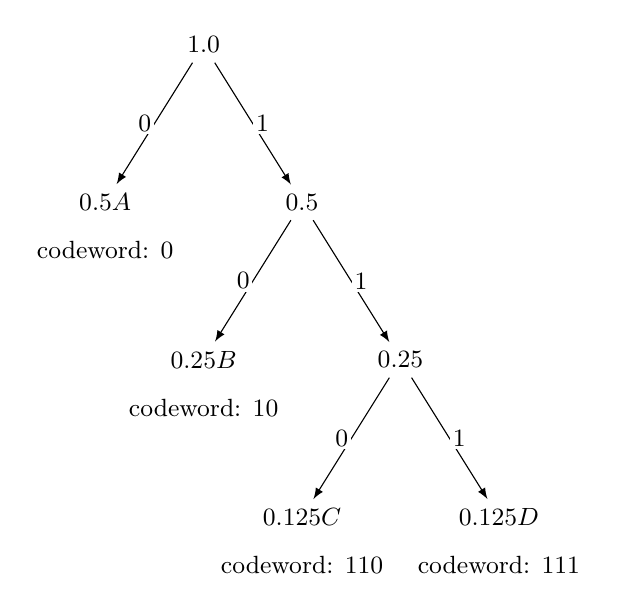
\begin{tikzpicture}[
    level distance=20mm,
    sibling distance=25mm,
    edge from parent/.style={draw, -latex},
    every node/.style={font=\small},
    prob/.style={fill=white, inner sep=1pt}
]

% Root
\node (root) {1.0}
    child {node (A) {0.5 \\ $A$}
        edge from parent node[prob,left] {0}
    }
    child {node (Bnode) {0.5}
        child {node (B) {0.25 \\ $B$}
            edge from parent node[prob,left] {0}
        }
        child {node (CD) {0.25}
            child {node (C) {0.125 \\ $C$}
                edge from parent node[prob,left] {0}
            }
            child {node (D) {0.125 \\ $D$}
                edge from parent node[prob,right] {1}
            }
            edge from parent node[prob,right] {1}
        }
        edge from parent node[prob,right] {1}
    };

% Add codeword labels below leaves
\node[below=4pt of A] {codeword: 0};
\node[below=4pt of B] {codeword: 10};
\node[below=4pt of C] {codeword: 110};
\node[below=4pt of D] {codeword: 111};

\end{tikzpicture}











Consider a source with four symbols and the following distribution:
\[
P(A) = 0.5,\quad P(B) = 0.25,\quad P(C) = 0.125,\quad P(D) = 0.125.
\]

\textbf{Step 1:} Combine the two least likely symbols, \(C\) and \(D\) (total probability \(0.25\)). \\
\textbf{Step 2:} Combine this new node with \(B\) (both \(0.25\)) to form a node of probability \(0.5\). \\
\textbf{Step 3:} Finally, combine with \(A\) (\(0.5\)) to complete the tree.

Assigning 0 to left branches and 1 to right branches yields the codewords:
\[
A \to 0,\quad B \to 10,\quad C \to 110,\quad D \to 111.
\]

The average code length is:
\[
L_{\text{avg}} = 0.5(1) + 0.25(2) + 0.125(3) + 0.125(3) = 1.75 \text{ bits/symbol}.
\]

The entropy of the source is:
\[
H = -\big[0.5\log_2 0.5 + 0.25\log_2 0.25 + 2\cdot0.125\log_2 0.125\big] = 1.75 \text{ bits/symbol}.
\]

Here, Huffman coding \textbf{achieves the entropy exactly} because all probabilities are inverse powers of two—a rare but illustrative case.

In general, Huffman coding satisfies:
\[
H(P) \leq L_{\text{avg}} < H(P) + 1.
\]
Thus, it is optimal for single-symbol coding but may fall short of the entropy by up to one bit per symbol. However, by applying Huffman coding to \textbf{blocks of \(n\) symbols}, the average length per symbol can be made arbitrarily close to \(H(P)\) as \(n \to \infty\), thereby fulfilling Shannon’s promise.

In summary, \textbf{Shannon’s source coding theorem defines the ultimate limit of compression}, while \textbf{Huffman encoding provides an efficient, constructive method} that approaches this limit in practice. Together, they form the theoretical and algorithmic backbone of modern lossless compression—from ZIP files to PNG images.













\section{KL-divergence}








The Kullback--Leibler (KL) divergence, or relative entropy, is a cornerstone of information theory and statistical inference. It provides a precise way to quantify how one distribution differs from another. 

It is important to note that KL-divergence is not a true distance metric because it is not symmetric and does not satisfy the triangle inequality. Nevertheless the concept KL divergence is extremely useful in information theory, statistics and machine learning.

We will only be interested in the discrete case.

\subsection{Definition and Formula (Discrete Case)}

Let \( P \) and \( Q \) be two discrete probability distributions over the same finite or countable alphabet \( \mathcal{X} \). The KL divergence from \( Q \) to \( P \) is defined as:
\[
D_{\mathrm{KL}}(P \parallel Q) = \sum_{x \in \mathcal{X}} P(x) \log \frac{P(x)}{Q(x)}.
\]

We adopt the conventions:
\begin{itemize}
\item \( 0 \log \frac{0}{q} = 0 \) for any \( q \geq 0 \),
    \item \( p \log \frac{p}{0} = +\infty \) for any \( p > 0 \).
\end{itemize}

This ensures the divergence is well-defined and reflects the impossibility of assigning zero probability to an event that actually occurs under \( P \).

\subsection{Interpretation: Wasted Bits from Using the Wrong Code}

One of the most illuminating interpretations of KL divergence arises from Shannon’s source coding theorem. Suppose a source emits symbols according to the true distribution \( P \), but we design a prefix-free code assuming the distribution is \( Q \). The optimal expected code length for a symbol under the true distribution is the entropy:
\[
H(P) = -\sum_{x} P(x) \log P(x).
\]

However, if we encode using a code optimized for \( Q \), the expected length becomes:
\[
\mathbb{E}_P[-\log Q(X)] = -\sum_{x} P(x) \log Q(x).
\]

The difference between these two expectations is exactly the KL divergence:
\[
D_{\mathrm{KL}}(P \parallel Q) = \mathbb{E}_P[-\log Q(X)] - H(P).
\]
Indeed,
\begin{eqnarray*}
\mathbb{E}_P[-\log Q(X)] - H(P) 
&=& -\sum_x P(x) \log Q(x) + \sum_x P(x) \log P(x) \\
&=& \sum_x P(x) \bigl( \log P(x) - \log Q(x) \bigr) \\
&=& \sum_x P(x) \log \frac{P(x)}{Q(x)} \\
&=& D_{\mathrm{KL}}(P \parallel Q).
\end{eqnarray*}

Thus, \textbf{KL divergence measures the average number of extra bits per symbol wasted by encoding data from \( P \) using a code built for \( Q \)}. This inefficiency is always non-negative (Gibbs’ inequality), and it vanishes only when \( P = Q \).


\subsection{Connection to Conditional Entropy and Mutual Information}

KL divergence is intimately linked to other core information-theoretic quantities. A key example is \textbf{mutual information} between two discrete random variables \( X \) and \( Y \). Mutual information can be expressed as a KL divergence between the joint distribution \( P_{X,Y} \) and the product of the marginals \( P_X P_Y \):
\[
I(X;Y) = D_{\mathrm{KL}}\big(P_{X,Y} \parallel P_X P_Y\big).
\]

This shows that mutual information quantifies how much the joint behavior of \( X \) and \( Y \) deviates from statistical independence.

Alternatively, mutual information is also given by the reduction in uncertainty:
\[
I(X;Y) = H(X) - H(X|Y),
\]
where the \textbf{conditional entropy} \( H(X|Y) \) is defined as:
\[
H(X|Y) = -\sum_{x,y} P(x,y) \log P(x|y).
\]

The connection between these two expressions becomes clear when we expand the KL divergence:
\begin{align*}
I(X;Y) &= D_{\mathrm{KL}}\big(P_{X,Y} \parallel P_X P_Y\big) \\
&= \sum_{x,y} P(x,y) \log \frac{P(x,y)}{P(x)P(y)} \\
&= \sum_{x,y} P(x,y) \log \frac{P(x|y)}{P(x)} \\
&= \sum_{x,y} P(x,y) \big[ \log P(x|y) - \log P(x) \big] \\
&= \underbrace{-\sum_{x,y} P(x,y) \log P(x)}_{H(X)} \;-\; \underbrace{\big(-\sum_{x,y} P(x,y) \log P(x|y)\big)}_{H(X|Y)} \\
&= H(X) - H(X|Y).
\end{align*}

This derivation reveals that the KL divergence formulation and the conditional entropy formulation are mathematically identical—just two perspectives on the same quantity. The KL view emphasizes \textbf{dependence as deviation from independence}, while the entropy view emphasizes \textbf{information gain through observation}.

\subsection{Conclusion}

In the discrete setting, KL divergence serves as a rigorous measure of informational inefficiency and distributional mismatch. Whether interpreted as wasted bits in coding, a tool for model selection, or the foundation of mutual information, it provides a unifying framework for understanding uncertainty and dependence. Its asymmetry is not a limitation but a reflection of the directional nature of information loss: assuming the wrong model has consequences that depend critically on which distribution is ``true'' and which is ``assumed.'' As such, KL divergence remains indispensable in information theory, statistics, and modern machine learning.







\section*{Information Gain from Bayesian Updating}

Mutual information and Bayes' theorem are deeply connected:
\begin{itemize}
\item \textbf{Bayes' theorem} tells you how to update a \emph{single prior} \(P(X)\) to a \emph{posterior} \(P(X \mid Y = y)\) after observing a specific outcome \(Y = y\).
    \item \textbf{Mutual information} \(I(X;Y)\) tells you the \emph{expected reduction in uncertainty} about \(X\) \emph{on average} over all possible outcomes \(y\), weighted by their likelihood.
\end{itemize}


In short:
\begin{center}
    \textbf{Mutual information = Expected information gain from Bayesian updating.}
\end{center}

\section*{Formal Connection}

\subsection*{1. Bayes' Theorem and Information Gain for a Single Observation}

Given a prior distribution \(P(X)\), observing \(Y = y\) yields the posterior via Bayes' rule:
\[
P(X \mid Y = y) = \frac{P(Y = y \mid X)\, P(X)}{P(Y = y)}.
\]

The \textbf{information gained} from this observation is measured by the Kullback–Leibler (KL) divergence from the prior to the posterior:
\[
D_{\mathrm{KL}}\big(P(X \mid Y = y) \,\|\, P(X)\big) 
= \sum_{x} P(x \mid y) \log_2 \frac{P(x \mid y)}{P(x)}.
\]
This quantifies how much the belief about \(X\) changed due to seeing \(Y = y\).

\subsection*{2. Mutual Information as Expected KL Divergence}

Mutual information is the expectation of this KL divergence over all possible outcomes \(y\):
\[
\boxed{
I(X;Y) = \mathbb{E}_{Y}\!\left[ D_{\mathrm{KL}}\big(P(X \mid Y) \,\|\, P(X)\big) \right]
= \sum_{y} P(y) \sum_{x} P(x \mid y) \log_2 \frac{P(x \mid y)}{P(x)}.
}
\]

Using \(P(x,y) = P(x \mid y) P(y)\), this is algebraically equivalent to the standard definition:
\[
I(X;Y) = \sum_{x,y} P(x,y) \log_2 \left( \frac{P(x,y)}{P(x) P(y)} \right).
\]

Thus, mutual information is precisely the \textbf{average information gain} from applying Bayes' rule.

\section*{Interpretation}


\begin{itemize}
    \item \textbf{KL divergence} \(D_{\mathrm{KL}}(P(X|y) \| P(X))\): \\
    ``How many extra bits would I waste if I encoded \(X\) using the prior instead of the correct posterior?'' \\
    This is the \emph{information gained} from observing \(Y = y\).

    \item \textbf{Mutual information} \(I(X;Y)\): \\
    ``On average, how many bits do I gain about \(X\) per observation of \(Y\)?'' \\
    This is the \emph{expected information gain} from Bayesian updating.
\end{itemize}

\subsection{Concrete Dice Example: Connecting Bayes + Mutual Information}

Recall the setup:
\begin{itemize}
\item Roll two fair dice: \(D_1, D_2\).
    \item Let \(X = D_1\) (first die), \(Y = D_1 + D_2\) (sum).
    \item Prior: \(P(X = x) = \frac{1}{6}\) for \(x = 1,\dots,6\).
\end{itemize}






\subsection*{Bayesian Updating for Specific Observations}

\begin{enumerate}
    \item \textbf{Observe \(Y = 2\)}: \\
    Only possible if \(D_1 = 1, D_2 = 1\). \\
    Posterior: \(P(X = 1 \mid Y = 2) = 1\), others 0. \\
    Information gain:
    \[
    D_{\mathrm{KL}}(P(X|2) \| P(X)) = \log_2 \frac{1}{1/6} = \log_2 6 \approx 2.585 \text{ bits}.
    \]

    \item \textbf{Observe \(Y = 7\)}: \\
    All pairs \((1,6), (2,5), \dots, (6,1)\) equally likely. \\
    Posterior: \(P(X = x \mid Y = 7) = \frac{1}{6}\) for all \(x\). \\
    Information gain:
    \[
    D_{\mathrm{KL}}(P(X|7) \| P(X)) = \sum_{x=1}^6 \frac{1}{6} \log_2 \frac{1/6}{1/6} = 0 \text{ bits}.
    \]
\end{enumerate}

\subsection*{Mutual Information as the Average Gain}

Mutual information averages these gains over all possible sums:
\[
I(X;Y) = \sum_{y=2}^{12} P(Y = y) \cdot D_{\mathrm{KL}}\big(P(X \mid Y = y) \,\|\, P(X)\big).
\]

Using the known distribution of \(Y\):
\begin{center}
\begin{tabular}{c|ccccccccccc}
\(y\) & 2 & 3 & 4 & 5 & 6 & 7 & 8 & 9 & 10 & 11 & 12 \\
\midrule
\(P(Y=y)\) & \(\frac{1}{36}\) & \(\frac{2}{36}\) & \(\frac{3}{36}\) & \(\frac{4}{36}\) & \(\frac{5}{36}\) & \(\frac{6}{36}\) & \(\frac{5}{36}\) & \(\frac{4}{36}\) & \(\frac{3}{36}\) & \(\frac{2}{36}\) & \(\frac{1}{36}\) \\
\(n_y\) (support size) & 1 & 2 & 3 & 4 & 5 & 6 & 5 & 4 & 3 & 2 & 1 \\
\(D_{\mathrm{KL}}\) & \(\log_2 6\) & \(\log_2 3\) & \(\log_2 2\) & \(\log_2 \tfrac{4}{3}\)? & \dots & 0 & \dots & & & &
\end{tabular}
\end{center}

More precisely, since \(P(X \mid Y = y)\) is uniform over \(n_y\) values,
\[
D_{\mathrm{KL}}\big(P(X \mid Y = y) \,\|\, P(X)\big) = \log_2 n_y - \log_2 6 = \log_2 \left( \frac{n_y}{6} \right) \quad \text{(but note: actually } = \log_2 n_y \text{ because prior entropy cancels in expectation)}.
\]

Carrying out the full calculation (as in the earlier example) yields:
\[
I(X;Y) \approx 0.6895 \text{ bits}.
\]

This is exactly the \textbf{expected information gain} from observing the sum and applying Bayes' rule.

\section*{Why This Matters}

[leftmargin=*]\begin{itemize}
    \item \textbf{Bayesian inference}: Every Bayes update provides information; mutual information quantifies its average value.
    \item \textbf{Experimental design}: Choose observations \(Y\) that maximize \(I(X;Y)\) to learn most about \(X\).
    \item \textbf{Machine learning}: In variational inference, mutual information appears in bounds on model evidence.
    \item \textbf{Cognitive science}: Models perception as Bayesian updating, with mutual information measuring sensory informativeness.
\end{itemize}

\section*{Summary}

\begin{center}
\begin{tabular}{ll}
\toprule
Concept & Role \\
\midrule
Bayes' theorem & Updates prior \(P(X)\) → posterior \(P(X \mid Y = y)\) for a \emph{specific} \(y\). \\
KL divergence \(D_{\mathrm{KL}}(P(X|y) \| P(X))\) & Information gained from that \emph{specific} update. \\
Mutual information \(I(X;Y)\) & \emph{Expected} information gain over all \(y\). \\
\bottomrule
\end{tabular}
\end{center}

Thus, mutual information provides an \textbf{information-theoretic foundation for Bayesian learning}: it measures how much an observation is expected to teach us about the world.





\end{document}













\end{document}















\end{document}
